%4.	Opis algorytmu rojowego (rozróżnić co z literatury co sam wymyśliłem)
%a.	Test dla zwykłej funkcji

\chapter{Algorytmy rojowe} \label{algo}

Po ogólnym wprowadzeniu do tematu w rozdziale \ref{wstep}, czas przejść do omówienia zastosowanej metody. Jednym z bardziej rzucających się w oczy wyrażeń w tytule pracy jest "algorytmy rojowe" i to właśnie nimi zajmiemy się w tym rozdziale. Zostanie omówiona istota algorytmów rojowych, zarówno w literaturze jak i ostateczna wersja zastosowana w programie, oraz, na koniec, zostanie przedstawiony przykład implementacji na funkcji dwóch zmiennych.

%----------------------------------------------------------------------------------------
%----------------------------------------------------------------------------------------
%----------------------------------------------------------------------------------------

\section{Algorytmy rojowe w literaturze}

Algorytmy rojowe należą do rodziny algorytmów stadnych. Ich główną ideą jest wykorzystanie sposobu zachowywania się pszczół zwiadowców podczas zbierania nektaru. Pszczoły, zgodnie z \cite{algroj}, wyruszają na łąkę w poszukiwaniu kwiatów z dużą ilością nektaru. Następnie wracają do ula i wykonują tak zwany taniec pszczeli podczas którego dochodzi do wymiany informacji między pszczołami na temat lokalizacji kwiatów o dużej zawartości nektaru. To pozwala na wysłanie pozostałych pszczół (czyli tych, które nie znalazły dobrych źródeł nektaru) do najlepszych lokalizacji. Im źródło zawiera więcej nektaru, tym więcej pszczół kieruje się do niego.

W literaturze (\cite{algroj}, \cite{algroj2}, \cite{algroj3}) można znaleźć różne opisy funkcjonowania tych algorytmów. Podejście różni się od źródła do źródła, lecz ogólny przebieg algorytmu rojowego jest taki sam i przedstawia się następująco:
\newpage
\begin{enumerate}
    \setcounter{enumi}{-1}
    \item inicjalizacja parametrów przekazanych programowi przy uruchomieniu:
     \begin{itemize}
        \item[$w_{best}$] - współczynnik określający procent rozwiązań uważanych za najlepsze względem wszystkich rozwiązań,
        \item[$w_{qual}$] - współczynnik określający procent rozwiązań uważanych za dobre względem wszystkich rozwiązań,
        \item[$w_{better}$] - współczynnik określający w jaki sposób pszczoły podzielą się na rozwiązania dobre i najlepsze. Jest to wartość z zakresu $(0, 1)$ i im jest większa tym więcej pszczół zostanie przydzielonych do przeszukiwania obszaru wokół rozwiązań najlepszych,
        \item[$d_{near}$] - wartość określająca odległość przeszukiwania od rozwiązania pierwotnego (sąsiedztwo),
        \item[$N$] - liczba pszczół zwiadowców biorąca udział w poszukiwaniu rozwiązania,
    \end{itemize}
     oraz zmiennych:
    \begin{itemize}
        \item[$n$] - liczba wszystkich rozwiązań,
        \item[$n_{best}$] - liczba najlepszych rozwiązań (w chwili początkowej$ = 0$) określona współczynnikiem $w_{best}$,
        \item[$n_{qual}$] - liczba rozwiązań dobrych (w chwili początkowej$ = 0)$ określona współczynnikiem $w_{qual}$,
        \item[$n_{left}$] - liczba rozwiązań pozostałych (nie zdefiniowanych jako dobre lub najlepsze) (w chwili początkowej$ = 0$),
    \end{itemize}
   \label{e1}
   \item wygenerowanie początkowych $N$ rozwiązań,
    \item ocena znalezionych rozwiązań przy użyciu funkcji celu, podział ich na kategorie (najlepsze, dobre i pozostałe lub dobre i pozostałe), \label{e2}
    \item przeszukiwanie sąsiedztwa najlepszych znalezionych rozwiązań w promieniu $d_{near}$ od danego rozwiązania, \label{e3}
     \item wybranie najlepszego rozwiązania z każdej przeszukiwanej lokalizacji, \label{e4}
    \item zapisanie najlepszego rozwiązania, \label{e5}
    \item generacja nowej populacji rozwiązań w zadanym obszarze, uwzględniając te znalezione w etapie \ref{e3}, tak aby ich liczba osiągnęła $N$, \label{e6} 
    \item powrót do etapu \ref{e2} lub zakończenie działania programu w przypadku spełnienia warunku stopu.\label{e7}
\end{enumerate}

W celu lepszego zilustrowanie działania algorytmu zostały wykonane schematy na rysunku \ref{fig:schemat_roj}. Przebieg przedstawiony tam odpowiada dokładnie temu opisanemu w \cite{algroj}.

\begin{figure} [htbp]
    \centering
    \begin{subfigure}[b]{0.32\textwidth}
    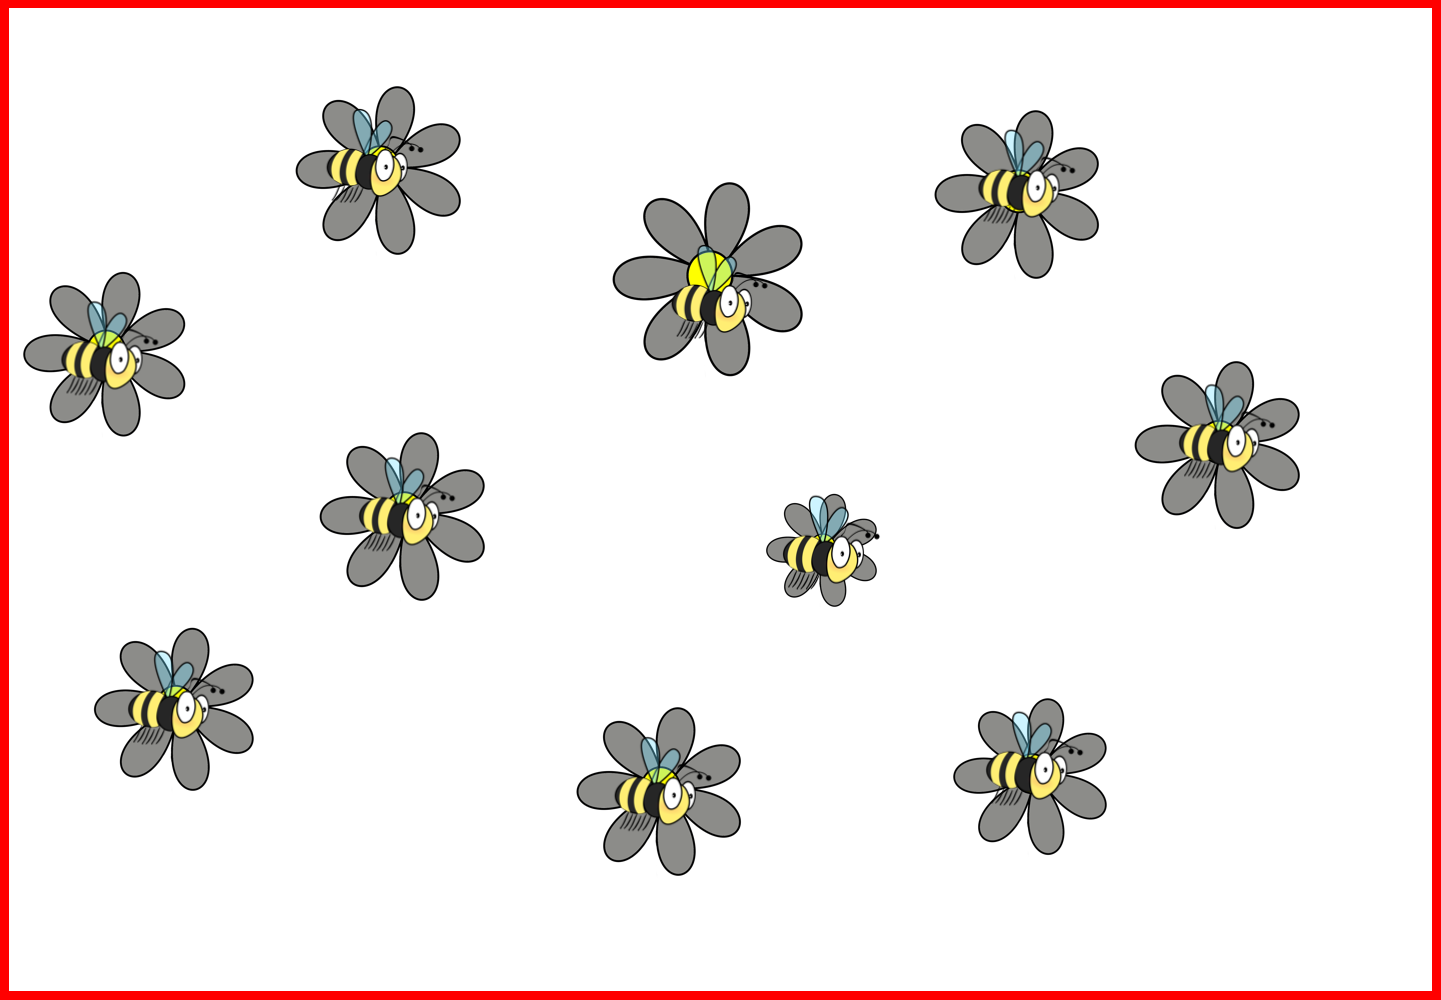
\includegraphics[width=\linewidth]{figures/rojowe/etap2.png}
    \caption{Losowanie rozwiązań\\~\\~\\~}
    \end{subfigure}
    \begin{subfigure}[b]{0.32\textwidth}
    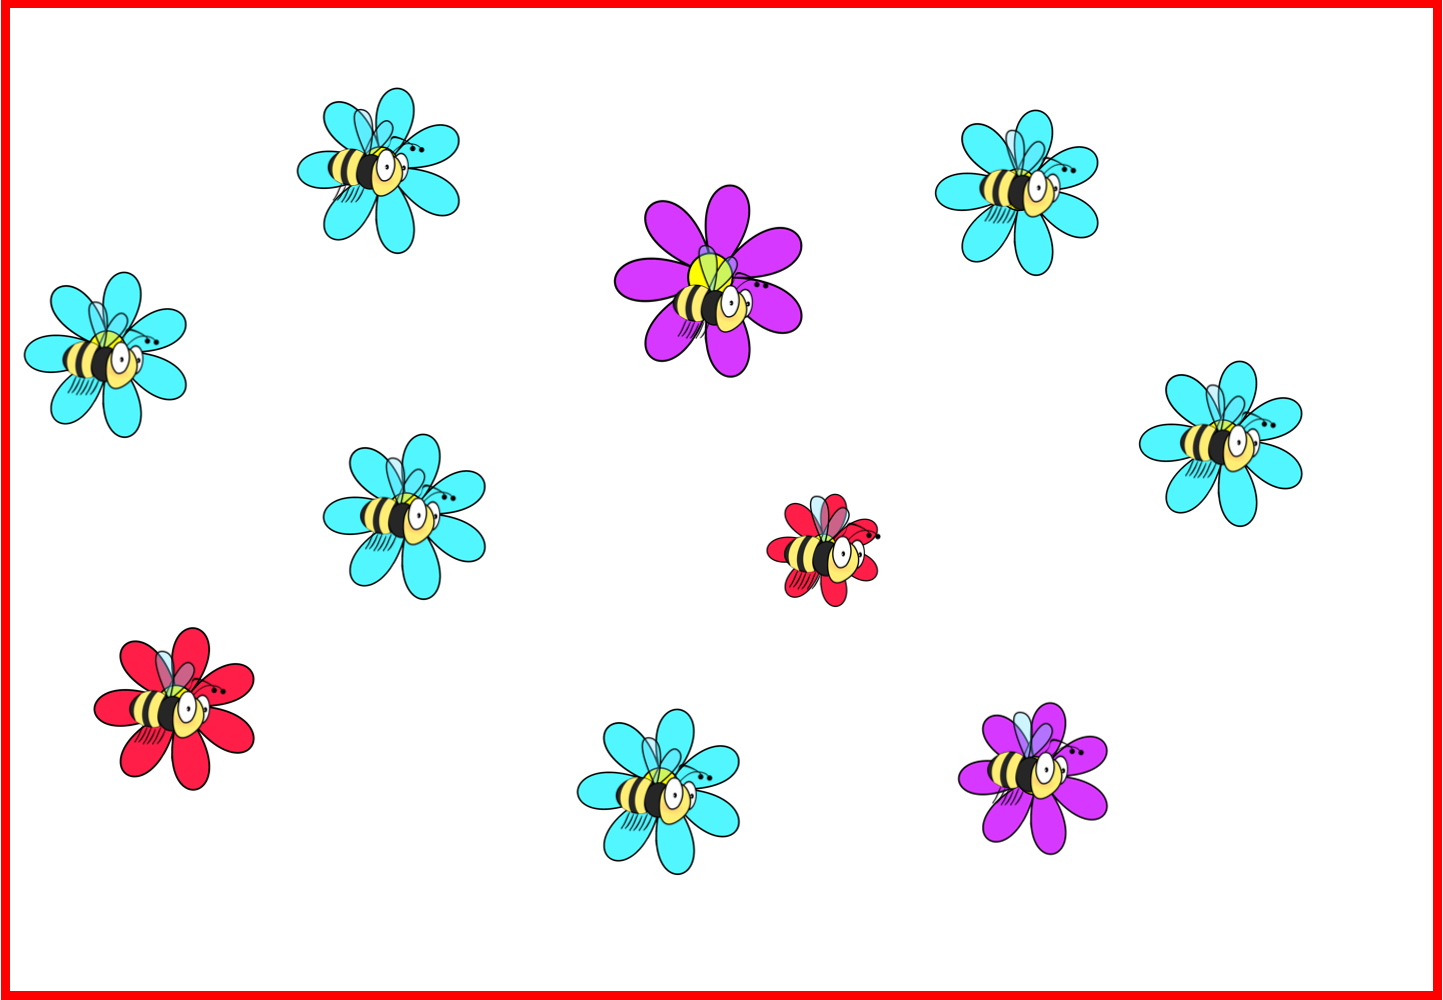
\includegraphics[width=\linewidth]{figures/rojowe/etap3.png}
    \caption{Ocena rozwiązań\\~\\~\\~}
    \end{subfigure}
    \begin{subfigure}[b]{0.32\textwidth}
    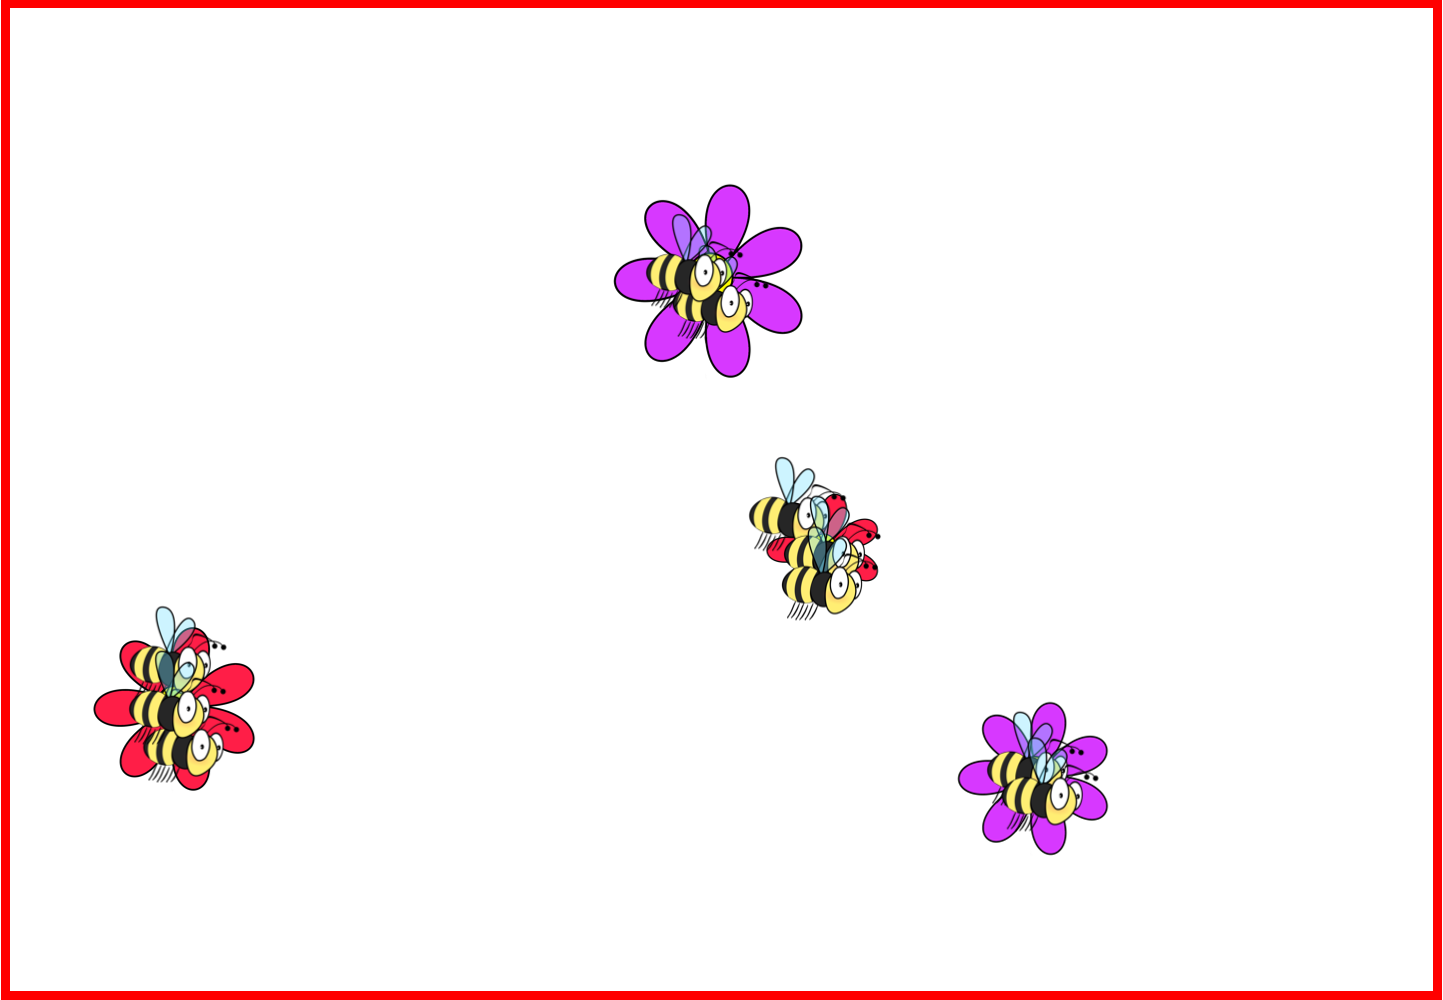
\includegraphics[width=\linewidth]{figures/rojowe/etap4.png}
    \caption{Przydział pszczół do rozwiązań dobrych i najlepszych oraz porzucenie pozostałych rozwiązań}
    \end{subfigure}
    \begin{subfigure}[b]{0.32\textwidth}
    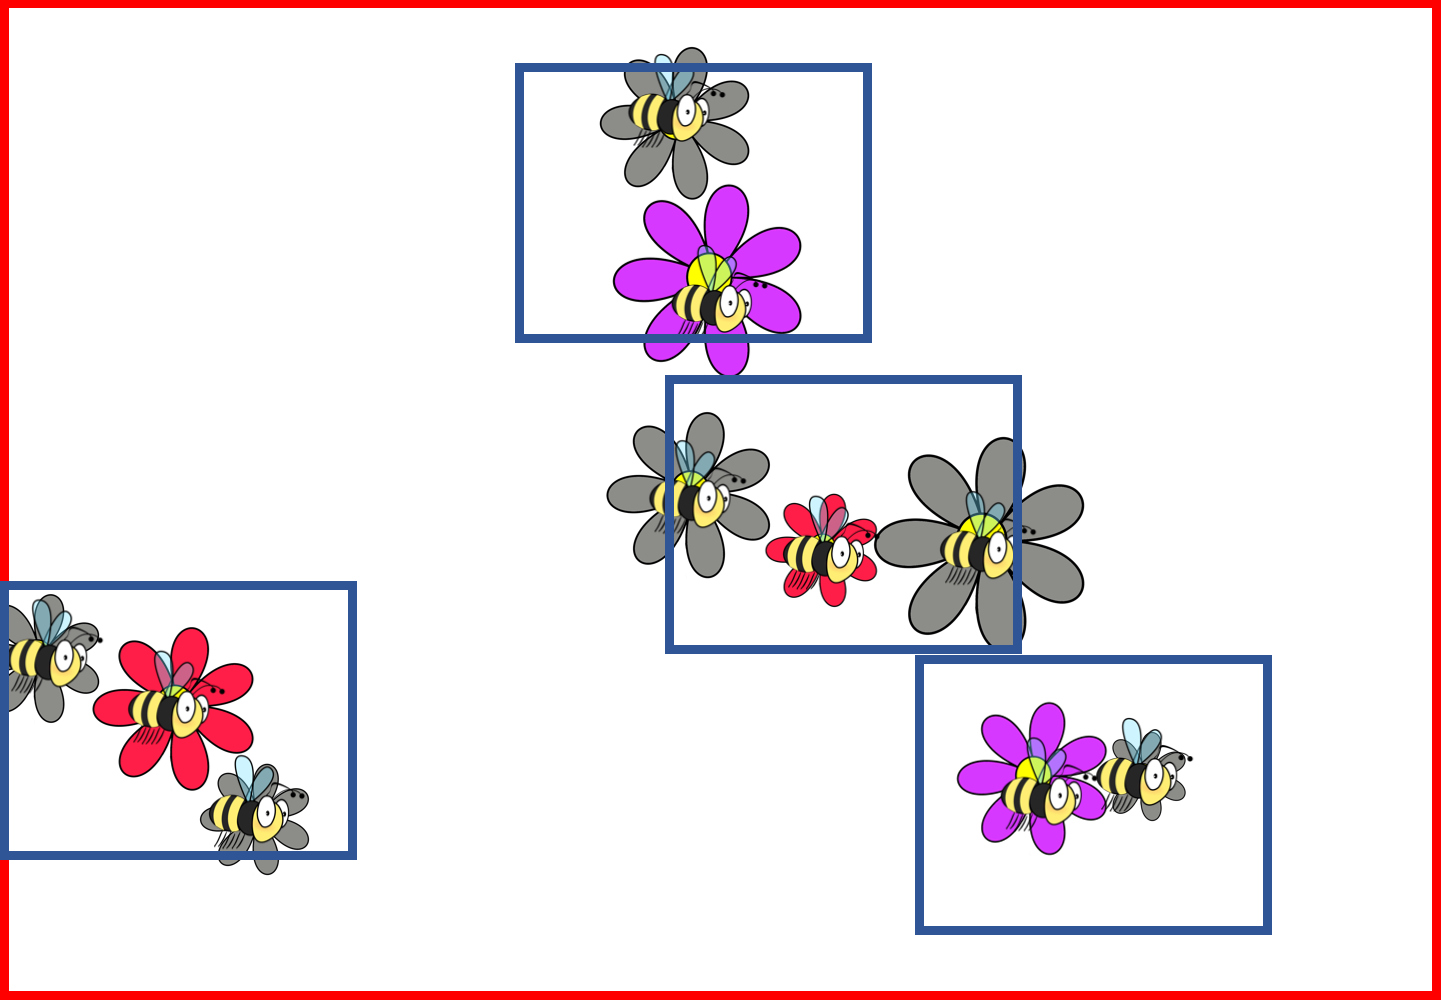
\includegraphics[width=\linewidth]{figures/rojowe/etap5.png}
    \caption{Losowanie rozwiązań w sąsiedztwie rozwiązań, które pozostały}
    \end{subfigure}
    \begin{subfigure}[b]{0.32\textwidth}
    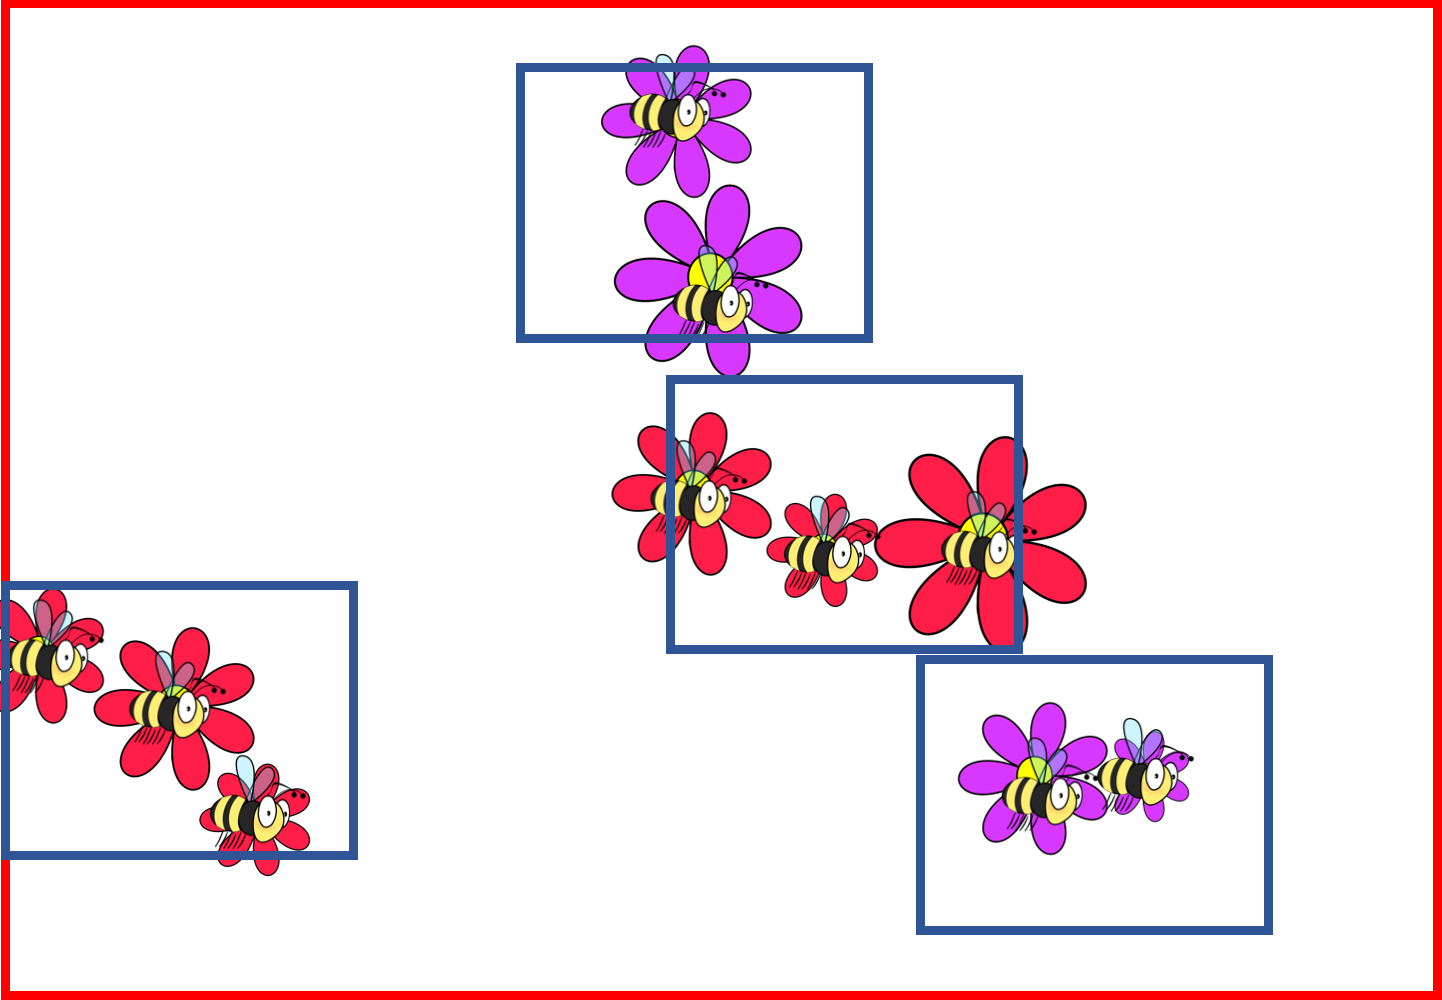
\includegraphics[width=\linewidth]{figures/rojowe/etap6.png}
    \caption{Ocena rozwiązań z sąsiedztwa\\~}
    \end{subfigure}
    \begin{subfigure}[b]{0.32\textwidth}
    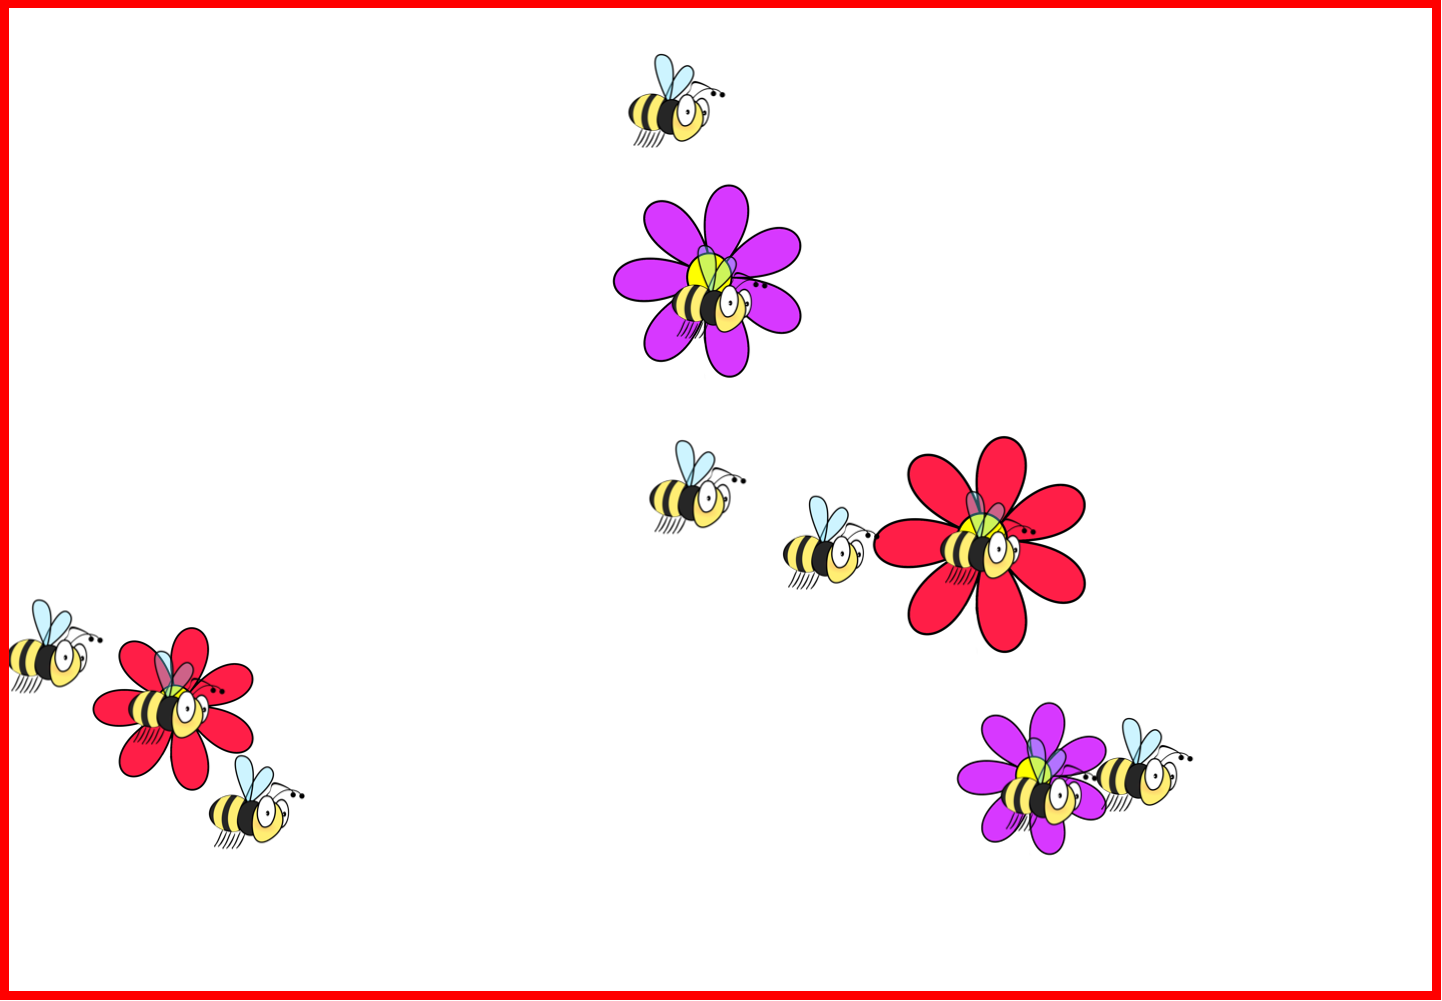
\includegraphics[width=\linewidth]{figures/rojowe/etap7.png}
    \caption{Wybór najlepszego rozwiązania z każdego obszaru}
    \end{subfigure}
    \begin{subfigure}[b]{0.32\textwidth}
    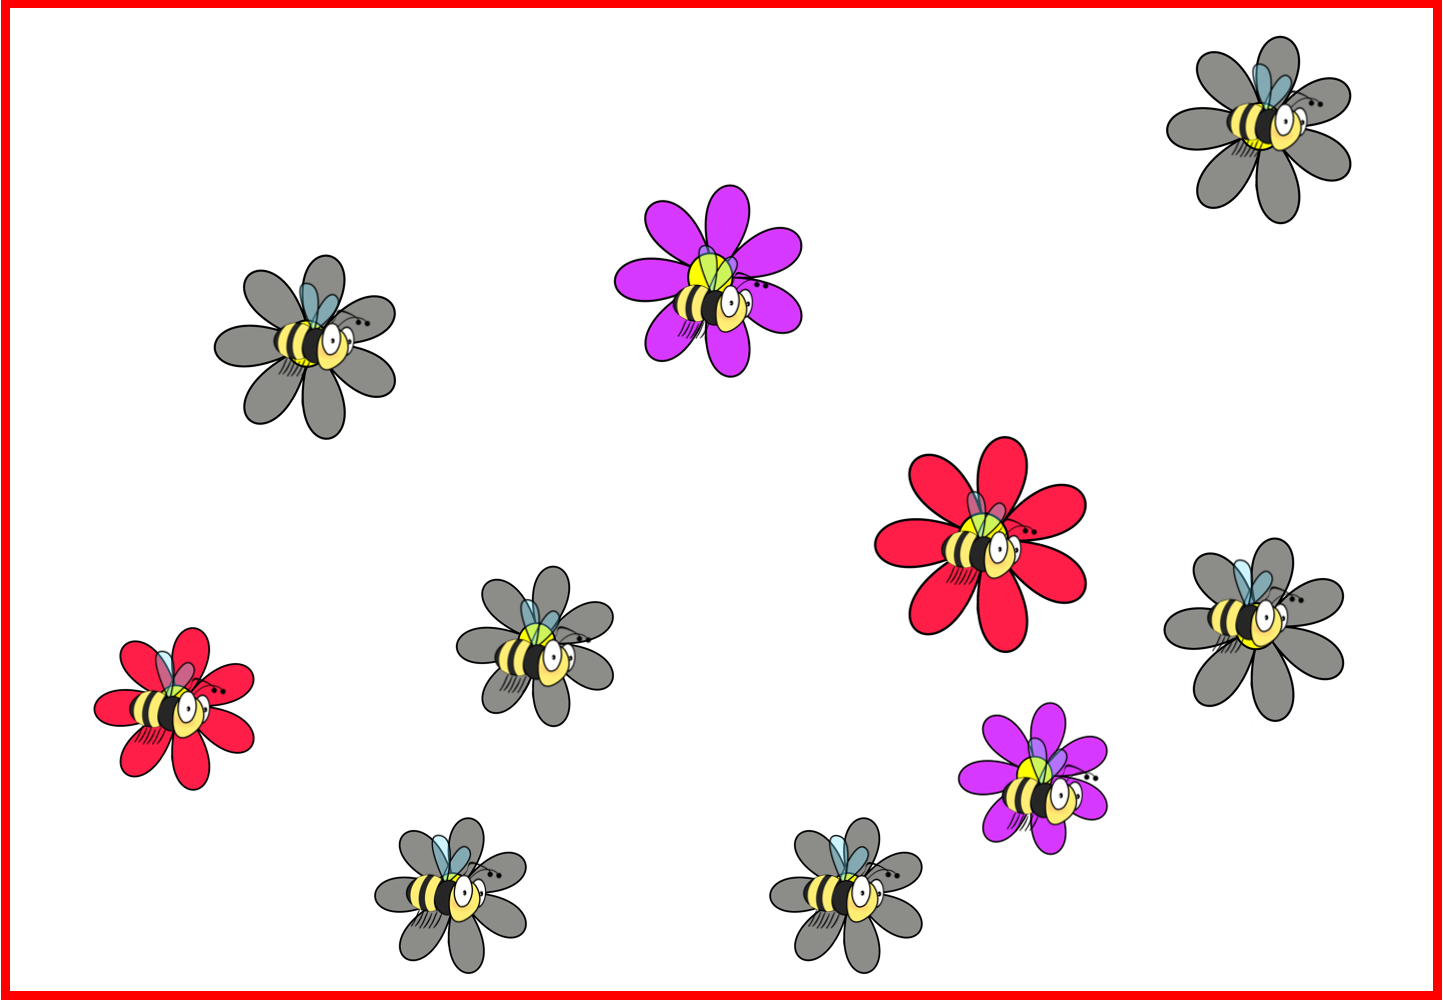
\includegraphics[width=\linewidth]{figures/rojowe/etap8.png}
    \caption{Pszczoły, które nie znalazły najlepszych rozwiązań, zostają przydzielone do nowych losowych rozwiązań}
    \end{subfigure}
    \begin{subfigure}[b]{0.32\textwidth}
    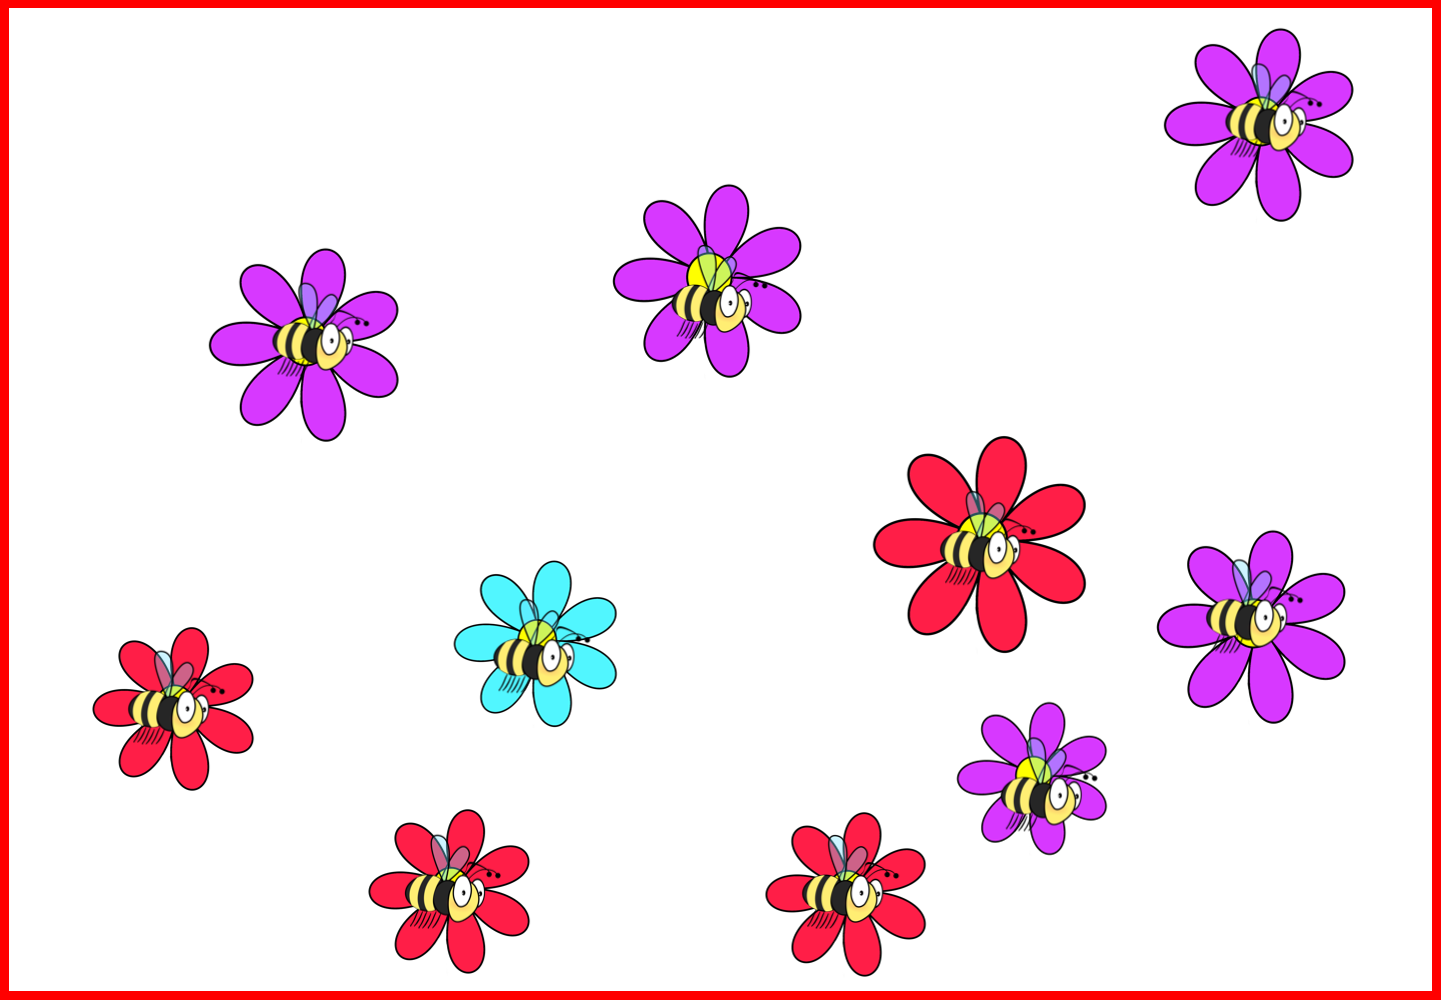
\includegraphics[width=\linewidth]{figures/rojowe/etap9.png}
    \caption{Ocena tak znalezionych rozwiązań\\~\\~\\~}
    \end{subfigure}
    \caption[Ilustrowany schemat działania algorytmu rojowego]{Ilustrowany schemat działania algorytmu rojowego zgodnie z \cite{algroj}.} 
    Oznaczenia: kwiatek czerwony --- rozwiązanie najlepsze, kwiatek fioletowy --- rozwiązanie dobre, kwiatek błękitny --- rozwiązanie z grupy pozostałych, czerwony prostokąt --- obszar losowania rozwiązań, niebieski prostokąt --- obszar sąsiedztwa danego rozwiązania, rozmiar kwiatka świadczy o jakości rozwiązania w swojej kategorii, tj. im kwiatek większy tym rozwiązanie lepsze.
    \label{fig:schemat_roj}
\end{figure}

Wszelkie różnice pojawiają się w szczegółowym przebiegu poszczególnych etapów. Pierwsza taka zauważalna różnica pojawia się w etapie \ref{e2}, gdzie niektóre źródła (\cite{algroj} i \cite{algroj3}) proponują podział ocenionych rozwiązań na dobre i najlepsze na podstawie parametrów $w_{best}$ i $w_{qual}$. W \cite{algroj} te parametry oznaczają wartość funkcji celu od jakiej dane rozwiązanie jest rozumiane jako dobre lub elitarne, natomiast w \cite{algroj3} są to parametry które określają procent rozwiązań z danej kategorii względem wszystkich rozwiązań. Inne źródła (\cite{algroj2}) proponują posortowanie rozwiązań od najlepszego do najgorszego bez rozróżniania najlepszych i elitarnych. Następnie, w etapie \ref{e3}, przy przeszukiwaniu rozwiązań, w \cite{algroj} i \cite{algroj3} przydziela się odpowiednią ilość pszczół zwiadowców do przeszukania sąsiedztwa danego rozwiązania w zależności od rangi rozwiązania (elitarne bądź dobre) zgodnie z parametrem $w_{better}$. Ten parametr ilustruje stosunek ilości pszczół przypisanych do przeszukiwania sąsiedztwa rozwiązań dobrych i elitarnych. Natomiast w \cite{algroj2}, biorąc pod uwagę brak podziału na dobre i elitarne, pszczoły są przydzielane w równych proporcjach do rozwiązań, które zostały wyznaczone do przeszukania ich sąsiedztwa. Ponadto, etap \ref{e5} jest pominięty w \cite{algroj}, ale nie odgrywa on szczególnie ważnej roli, gdyż najlepszy wynik zawsze przechodzi do następnej iteracji i zawsze istnieje możliwość jego odczytania.

Z dodatkowych różnic można wspomnieć wprowadzenie długości życia rozwiązania w \cite{algroj3}. Ta długość życia miałaby pozwolić na wyeliminowanie rozwiązań, które będą się powtarzać przez określoną wcześniej liczbę iteracji.  

%----------------------------------------------------------------------------------------
%----------------------------------------------------------------------------------------
%----------------------------------------------------------------------------------------

\section{Algorytm zastosowany w programie}

Algorytm zastosowany w tejże pracy przeszedł parę delikatnych transformacji przez cały czas sporządzania finalnego modelu wartości dyspersyjnych zwierciadła DBR. Jako algorytm wejściowy został zastosowany ten opisany w \cite{algroj}. Na początku funkcja celu została zaprojektowana tak, aby zwracała wartości z zakresu (0,1). Rozwiązania elitarne i dobre były ustalane na podstawie porównania wartości zwróconej przez funkcję celu z dwoma parametrami algorytmu, określającymi próg, od którego rozwiązania jest uznawane za dobre i próg, od którego rozwiązanie jest uznawane za elitarne. Dla tak dobranych rozwiązań, w sposób losowy, były generowane rozwiązania z sąsiedztwa danego rozwiązania. Po etapie \ref{e5} polegającym na zapisaniu najlepszego rozwiązania, algorytm sprawdzał czy suma rozwiązań dobrych i elitarnych nie przekroczyła danego progu będącego parametrem algorytmu, jeśli tak, wówczas próg minimalnej wartości funkcji celu dla rozwiązań dobrych i elitarnych był zwiększany oraz rozmiar sąsiedztwa rozwiązań był zwężany. Dodanie tego etapu wynikało z chęci przyspieszenia dążenia algorytmu do rozwiązania i nie występuje on w żadnym z wymienionych źródeł.

Po wielu testach zauważono, iż algorytm napotyka problemy przy generowaniu rozwiązań spełniających próg rozwiązań dobrych i elitarnych. Większość rozwiązań otrzymywała ocenę równą zeru. Problem polegał na funkcji celu i trudności w otrzymaniu oceny umożliwiającej rozróżnienie jakości wszystkich wygenerowanych rozwiązań, przy zachowaniu skali oceny w zakresie (0,1). Ten fakt wynikał z tego, iż cel, który program miałby osiągnąć nie mógł zostać określony w sposób jednoznaczny, aby móc ustalić maksymalną wartość rozwiązań jakie zostaną wygenerowane. Dlatego też funkcja celu została zmodyfikowana w taki sposób aby wystawiać ocenę rozwiązania bez korzystania z jakiejkolwiek skali. Tak zbudowana funkcja celu jest w stanie rozróżnić między jakością każdego wygenerowanego rozwiązania, lecz bez możliwości jednoznacznego określenia maksymalnej i minimalnej oceny jaką może wystawić. Ten fakt spowodował konieczność modyfikacji algorytmu. Zamiast wyznaczania rozwiązań elitarnych i dobrych na podstawie progów, rozwiązania są teraz sortowane na podstawie wartości funkcji celu od najlepszego do najgorszego, tak jak w \cite{algroj3}. Następnie, na podstawie parametrów $w_{best}$ i $w_{qual}$ określającymi procent rozwiązań elitarnych i dobrych względem wszystkich rozwiązań, rozwiązania są kategoryzowane. Dla przykładu, jeżeli bierzemy pod uwagę $100$ rozwiązań i parametry $w_{best}$ i $w_{qual}$ wynoszą kolejno $0,1$ i $0,2$, po posortowaniu od najlepszego do najgorszego pierwsze 10 rozwiązań jest uznawane za najlepsze, natomiast 20 następnych rozwiązań jako dobre. Dalej przebieg wygląda tak samo jak w źródle \cite{algroj}.

W algorytmie dodatkowo dopuszczono generowanie rozwiązań początkowych w odległości $d_{far}$ od rozwiązania początkowego załadowanego z zewnątrz programu. Warto zauważyć, że $d_{far}$ jest dużo większe od $d_{near}$.

Finalny algorytm zastosowany w programie został zaprezentowany na rysunku \ref{fig:algorytm_koncowy}.

\begin{figure}[H]
    \centering
    \begin{tikzpicture}[node distance=2.5cm]
    \node (gen) [bullet] {Wygenerowanie $n$ rozwiązań};
    \node (ocen) [bullet, below of=gen] {Ocena wygenerowanych rozwiązań i ich posortowanie};
    \node (best) [bullet, below of=ocen, xshift=-100] {Przypisanie $n_{best} = w_{best}\cdot n$ pierwszych najlepszych rozwiązań do rozwiązań elitarnych};
    \node (qual) [bullet, below of=ocen,xshift=100] {Przypisanie $n_{qual} = w_{qual}\cdot n$ następnych najlepszych rozwiązań do rozwiązań dobrych};
    \node (beese) [bullet, below of=best] {Przypisanie $n_{best} = n_{best} + w_{better}\cdot n_{left}$ pszczół do przeszukiwania sąsiedztwa rozwiązań elitarnych};
    \node (beesm) [bullet, below of=qual] {Przypisanie $n_{qual} = n_{qual} + (1-w_{better})\cdot n_{left}$ pszczół do przeszukiwania sąsiedztwa rozwiązań dobrych};
    \node (ocena) [bullet, below of=beese,xshift=100] {Ocena znalezionych rozwiązań};
    \node (wybor) [bullet, below of=ocena] {Wybór jednego rozwiązania z każdej przeszukiwanej lokalizacji};
    \node (najlepszy) [bullet, below of=wybor] {Wybór najlepszego znalezionego rozwiązania};
    \node (cel) [bullet, below of=najlepszy,fill=yellow!30] {Czy warunek stopu spełniony?};
    \node (koniec) [bullet, below of=cel] {Koniec działania algorytmu. Zapis podsumowania do pliku};
    \node (konty) [bullet, below of=najlepszy,xshift=200, text width=0.2\linewidth] {Wygenerowanie $n-n_{best}-n_{qual}$ losowych rozwiązań};
    \draw [arrow] (konty) |- (ocen);
    \draw [arrow] (gen) -- (ocen);
    \draw [arrow] (ocen) -- (best);
    \draw [arrow] (ocen) -- (qual);
    \draw [arrow] (best) -- (beese);
    \draw [arrow] (qual) -- (beesm);
    \draw [arrow] (beese) -- (ocena);
    \draw [arrow] (beesm) -- (ocena);
    \draw [arrow] (ocena) -- (wybor);
    \draw [arrow] (wybor) -- (najlepszy);
    \draw [arrow] (najlepszy) -- (cel);
    \draw [arrow,, color=black!60!green] (cel) -- node[anchor=east, color=black!60!green] {TAK} (koniec);
    \draw [arrow, color=black!40!red] (cel) -- node[anchor=south, color=black!40!red] {NIE} (konty);
    \end{tikzpicture}
    \caption{Przebieg algorytmu rojowego zastosowanego w programie}
    \label{fig:algorytm_koncowy}
\end{figure}

%----------------------------------------------------------------------------------------
%----------------------------------------------------------------------------------------
%----------------------------------------------------------------------------------------

\section{Przykład zastosowania na funkcji prostej}
W celu sprawdzenia efektywności algorytmu zostały wykonane testy na prostej funkcji dwóch zmiennych. Została wybrana funkcja Ackleya o wzorze:
\begin{equation}
f(x,y) = -20\exp\left[-0.2\sqrt{0.5\left(x^{2}+y^{2}\right)}\right] -\exp\left[0.5\left(\cos 2\pi x + \cos 2\pi y \right)\right] + e + 20,
\end{equation}

ze względu na to iż charakteryzuje się falistym wykresem z dużą ilością minimów lokalnych o wartościach malejących przy oddalaniu się od punktu $(0, 0)$, w którym to też znajduje się minimum globalne funkcji o wartości 0. Dla lepszego zobrazowania tej charakterystycznej struktury, wykres funkcji Ackleya został zaprezentowany na rysunku \ref{fig:ackley}.

\begin{figure}[H]
    \centering
    \begin{tabular}{cc}
         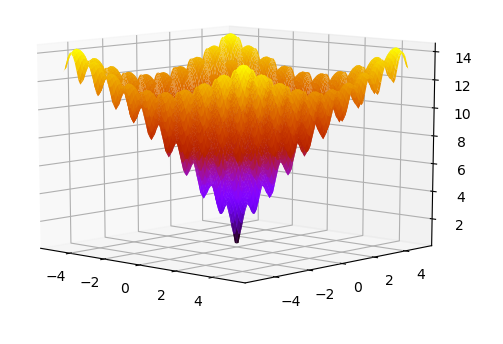
\includegraphics[width=0.5\linewidth]{figures/ackley1.png}& 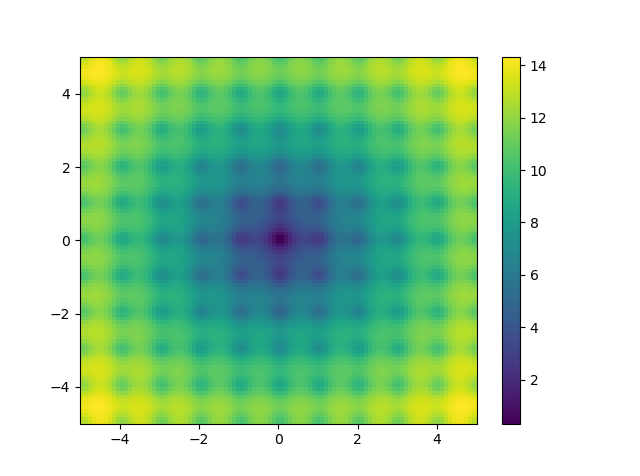
\includegraphics[width=0.5\linewidth]{figures/ackley2.png}
    \end{tabular}
    \caption{Funkcja Ackleya}
    \label{fig:ackley}
\end{figure}

Oprócz doboru badanej funkcji, bardzo istotnym elementem było określenie funkcji celu. W tym wypadku funkcja celu została zaprogramowana tak, że zwraca wartości z przedziału $\langle 0, 1 \rangle$ na podstawie modułu różnicy wartości funkcji od wartości $0$ w punkcie $(0, 0)$. Otrzymana liczba jest dzielona przez największą wartość jaką może przyjąć funckja w danych przedziale (w tej symulacji dla x i y w przedziale $\langle -1,5, 1,5\rangle$ maksymalna wartość funkcji wynosi $8$) i tak otrzymana liczba jest odejmowana od $1$ aby otrzymać skalę ocen w taki sposób, że im punkt bliższy rozwiązaniu tym ocena wyższa.

Symulacja została wykonana dla $N=1000$ zwiadowców, przy następujących wartościach parametrów: $d_{near} = 0,0005$, $w_{qual} = 0,20$, $w_{best} = 0,10$, $w_{better} = 0,6$. Wyniki obliczeń zostały przedstawione w tabeli \ref{tab:wyniki3d}.

\begin{table}[H]
    \centering
    \caption{Wyniki dla funkcji Ackleya}
    \begin{tabular}{cc}
         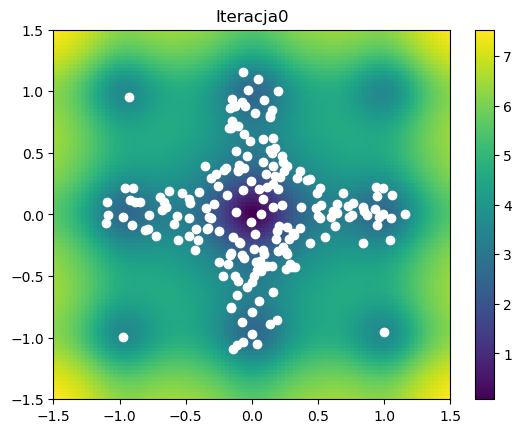
\includegraphics[width=0.5\linewidth]{figures/3d/it0.png} & 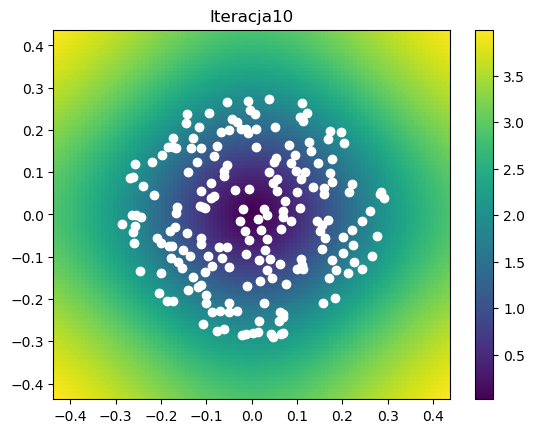
\includegraphics[width=0.5\linewidth]{figures/3d/it10.png} \\
         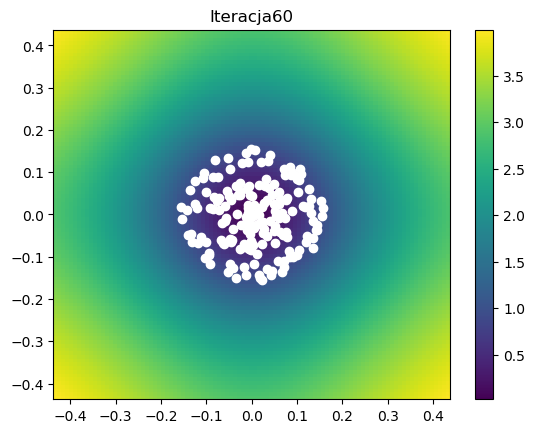
\includegraphics[width=0.5\linewidth]{figures/3d/it60.png} & 
         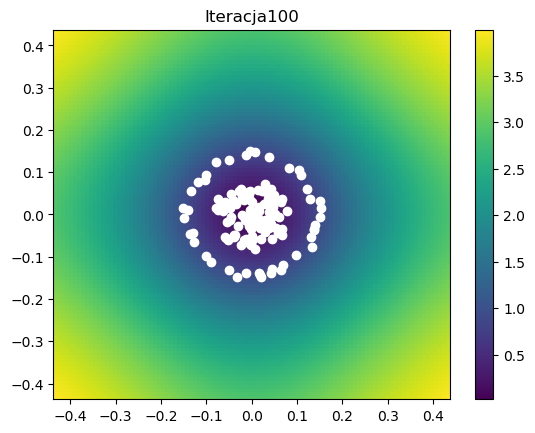
\includegraphics[width=0.5\linewidth]{figures/3d/it100.png} \\
         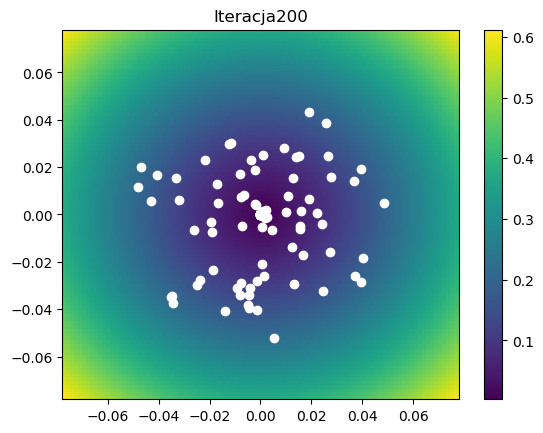
\includegraphics[width=0.5\linewidth]{figures/3d/it200.png} &
         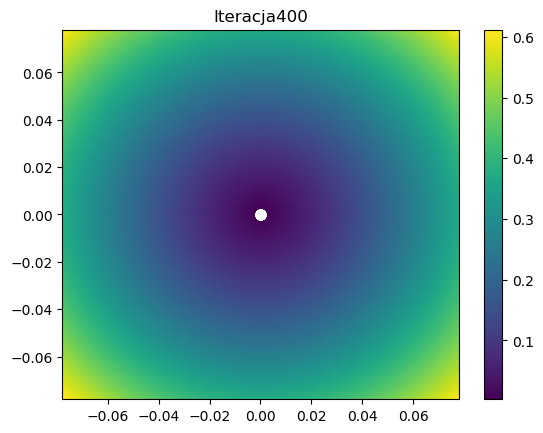
\includegraphics[width=0.5\linewidth]{figures/3d/it400.png}
    \end{tabular}
    \label{tab:wyniki3d}
\end{table}

Można zauważyć na podstawie wyników z tabeli \ref{tab:wyniki3d}, że z iteracji na iterację obszar poszukiwań zawęża się do coraz to bliższego sąsiedztwa poszukiwanego rozwiązania, dokładnie tak jak to było zamierzone. Dodatkowo otrzymany wynik po 400 iteracjach wynosi $6,32\cdot10^{-6}$ w punkcie ($-0,36\cdot10^{-6}$, $2,21\cdot10^{-6}$) co jest dobrym przybliżeniem szukanego rozwiązania.

Podsumowując algorytmy rojowe wydają się być dobrym narzędziem do rozwiązywania problemów w których celem jest odnalezienie minimum bądź maksimum danej funkcji. Algorytm wyznaczania struktury z najlepszymi właściwościami dyspersyjnymi jest właśnie poniekąd taką funkcją, której minimum będziemy próbowali znaleźć w następnym rozdziale.